% !TeX root = ../thuthesis-example.tex

\chapter{自主导航算法设计}

正如\ref{target}节所讲,本章要介绍的是一种基于强化学习的端到端自主导航算法。本章将首先介绍强化学习的基本概念以及本算法使用的骨干(Backbone)算法:近端梯度下降法(Prximal policy optimization, PPO),然后介绍自主导航算法的整体框架和神经网络结构设计,最后介绍本研究提出的三段式训练方法以及其它提升训练效果的手段。

\section{强化学习基本介绍}
强化学习是一类通过智能体与环境不断交互逐渐改进策略的机器学习方法。和有监督学习(Supervised Learning)不同,强化学习无需标签。本节将具体地介绍强化学习的基本概念、核心算法和本研究所使用的骨干算法:近端梯度下降法。

\subsection{强化学习基础}
强化学习中,智能体(Agent)是指执行学习和决策的实体,可以是一个机器人、自动驾驶车辆或其他能够感知环境、做出决策并执行动作的实体。环境(Environment)是智能体与之进行交互的外部实体,可以是真实的物理环境,也可以是仿真环境。
智能体在环境中有自身状态(State),并在观测到状态后选择一个动作(Action)。环境接受智能体的动作并执行、执行后为智能体生成奖励(Reward)。强化学习与环境交互的过程如图\ref{fig_RL}所示。

为方便阐述强化学习算法的设计,引入一些符号和标记。
\begin{enumerate}
  \item 强化学习将任务描述为一个离散的事件序列,每个事件称为一个时间步(Step),记为$t$。
  \item 在$t$时刻智能体观测到的状态记作$S_t$
  \item 智能体通过状态选择动作的方法称为策略,被记作$\pi(a|s)$描述在状态$s$下选择动作$a$的概率。
  \item $t$时刻根据智能体状态和动作由环境给出的及时反馈,记作$R_t$,是一个标量。通常由实验者手动设计。
\end{enumerate}
按照流程,若将初始值以角标$0$记录,不断交互就可以得到一条交互轨迹$\tau$:
\[
  S_0,\ R_0,\ A_0,\ S_1,\ R_1,\ A_1,\ S_2,\ R_2,\ A_2,\ \dots
\]
强化学习所研究的问题必须是马尔可夫决策(Markov Decision Process, MDP)问题,即下一时刻的状态仅仅与上一时刻的状态和动作有关,与之前的状态和动作无关。可以使用五元组$(\mathcal{S,A,P,R,}\gamma)$来描述MDP问题:
\begin{enumerate}
  \item $\mathcal{S}$为状态空间,表示所有可能出现的状态的集合。
  \item $\mathcal{A}$为动作空间,表示所有可能出现的动作的集合。
  \item $\mathcal{P}$为环境状态转移概率,表示给定某一时刻$(s,a)$下一时刻状态转移为$s'$的概率,即$\mathcal{P}(s'|s,a)$。
  \item $\mathcal{R}$为奖励函数,是$(s,a)$的函数。
  \item $\gamma$是折扣因子,$0\leq\gamma\leq 1$,表示智能体对未来奖励的重视程度。
\end{enumerate}

由此我们可以引出状态值函数(State value function)$V(s)$和动作值函数(Action value function)$Q(s,a)$的定义:
\[\begin{aligned}
  G_t &= \sum_{k=0}^{\infty} \gamma^k R_{t+k+1}\\
  V(s) &= \mathbb{E}[G_t|S_t=s]\\
  Q(s,a) &= \mathbb{E}[G_t|S_t=s,A_t=a]
\end{aligned}\]
MDP问题总存在最优策略$\pi^*$,满足
\[
  \pi^* = {\arg\max}_\pi {Q_\pi(s,a)}
\]
由于$\mathcal{P},\ \mathcal{R}$是智能体所未知的,因此强化学习的目的就是利用采集到的轨迹$\tau$更新策略$\pi$使得$\pi$尽可能接近$\pi^*$以获取最高的累计奖励$G_t$。其中通过估计值函数$V,\ Q$再通过值函数选择$a$的一类方法被称为基于值的方法(Value based) ,直接通过梯度更新策略$\pi$的一类方法被称为基于策略的方法(Policy Based)。

\subsection{近端策略优化算法}
\label{PPO_alg}
近端策略优化算法\cite{schulman2017proximal}(Prximal policy optimization, PPO)是一种Policy Based强化学习方法,并使用KL散度来控制策略的变化率使得策略始终保持在稳定的范围内。

PPO 算法采取Actor-Critic的训练架构,分别学习学习策略$\pi_\theta(a|s)$和价值函数$V_\phi(s)$,其中$\theta,\ \phi$分别是$\pi,\ \phi$的神经网络参数。PPO 算法的核心是使用一种称为“截断优化”(Clipping)的技术来限制策略更新的范围,以避免过大的策略更新幅度导致训练不稳定。PPO 的优化目标为:
\[
  J^{\mathrm{CLIP}}(\theta)=\mathbb{E}_{t}\left[\min \left(\alpha_{t}(\theta) \hat{A}_{t}, \operatorname{clip}\left(\alpha_{t}(\theta), 1-\epsilon, 1+\epsilon\right) \hat{A}_{t}\right)\right]
\]
其中
\[
  \alpha_{t}(\theta)=\frac{\pi_{\theta}\left(a_{t} \mid s_{t}\right)}{\pi_{\theta_{\text {old }}}\left(a_{t} \mid s_{t}\right)}
\]
表示新、旧策略之间的变化情况,$\epsilon$表示置信区间,$\hat{A}_t = G_t-V_{\pi_\theta}(s_t)$是优势函数(Advantage function).PPO 算法使用广义优势估计
(Generalized Advantage Estimation,GAE)[79]方法来估计$\hat{A}_t$。具体而言,GAE估计的公式如下:
\[
  A_{t}^{G A E(\gamma, \lambda)}=\sum_{l=0}^{\infty}(\gamma \lambda)^{l} \delta_{t+l}
\]
其中,$\delta_{t+1}$表示从时刻$t$开始的累计奖励与价值函数的差异:
\[
  \delta_{t+l}=r_{t+l}+\gamma V\left(s_{t+l+1}\right)-V\left(s_{t+l}\right)
\]
其中$\lambda$是一个超参数,控制GAE估计的偏差和方差间的权衡。在实践中,$\lambda$通常被设置为一个较小的值,例如$0.95$。

\section{端到端自主导航算法整体结构}
本研究设计了一套适用于无人机自主导航任务的端到端算法框架结构,如图\ref{fig_framework}所示。下面将详细介绍各部分的功能。
\begin{figure}
  \centering
  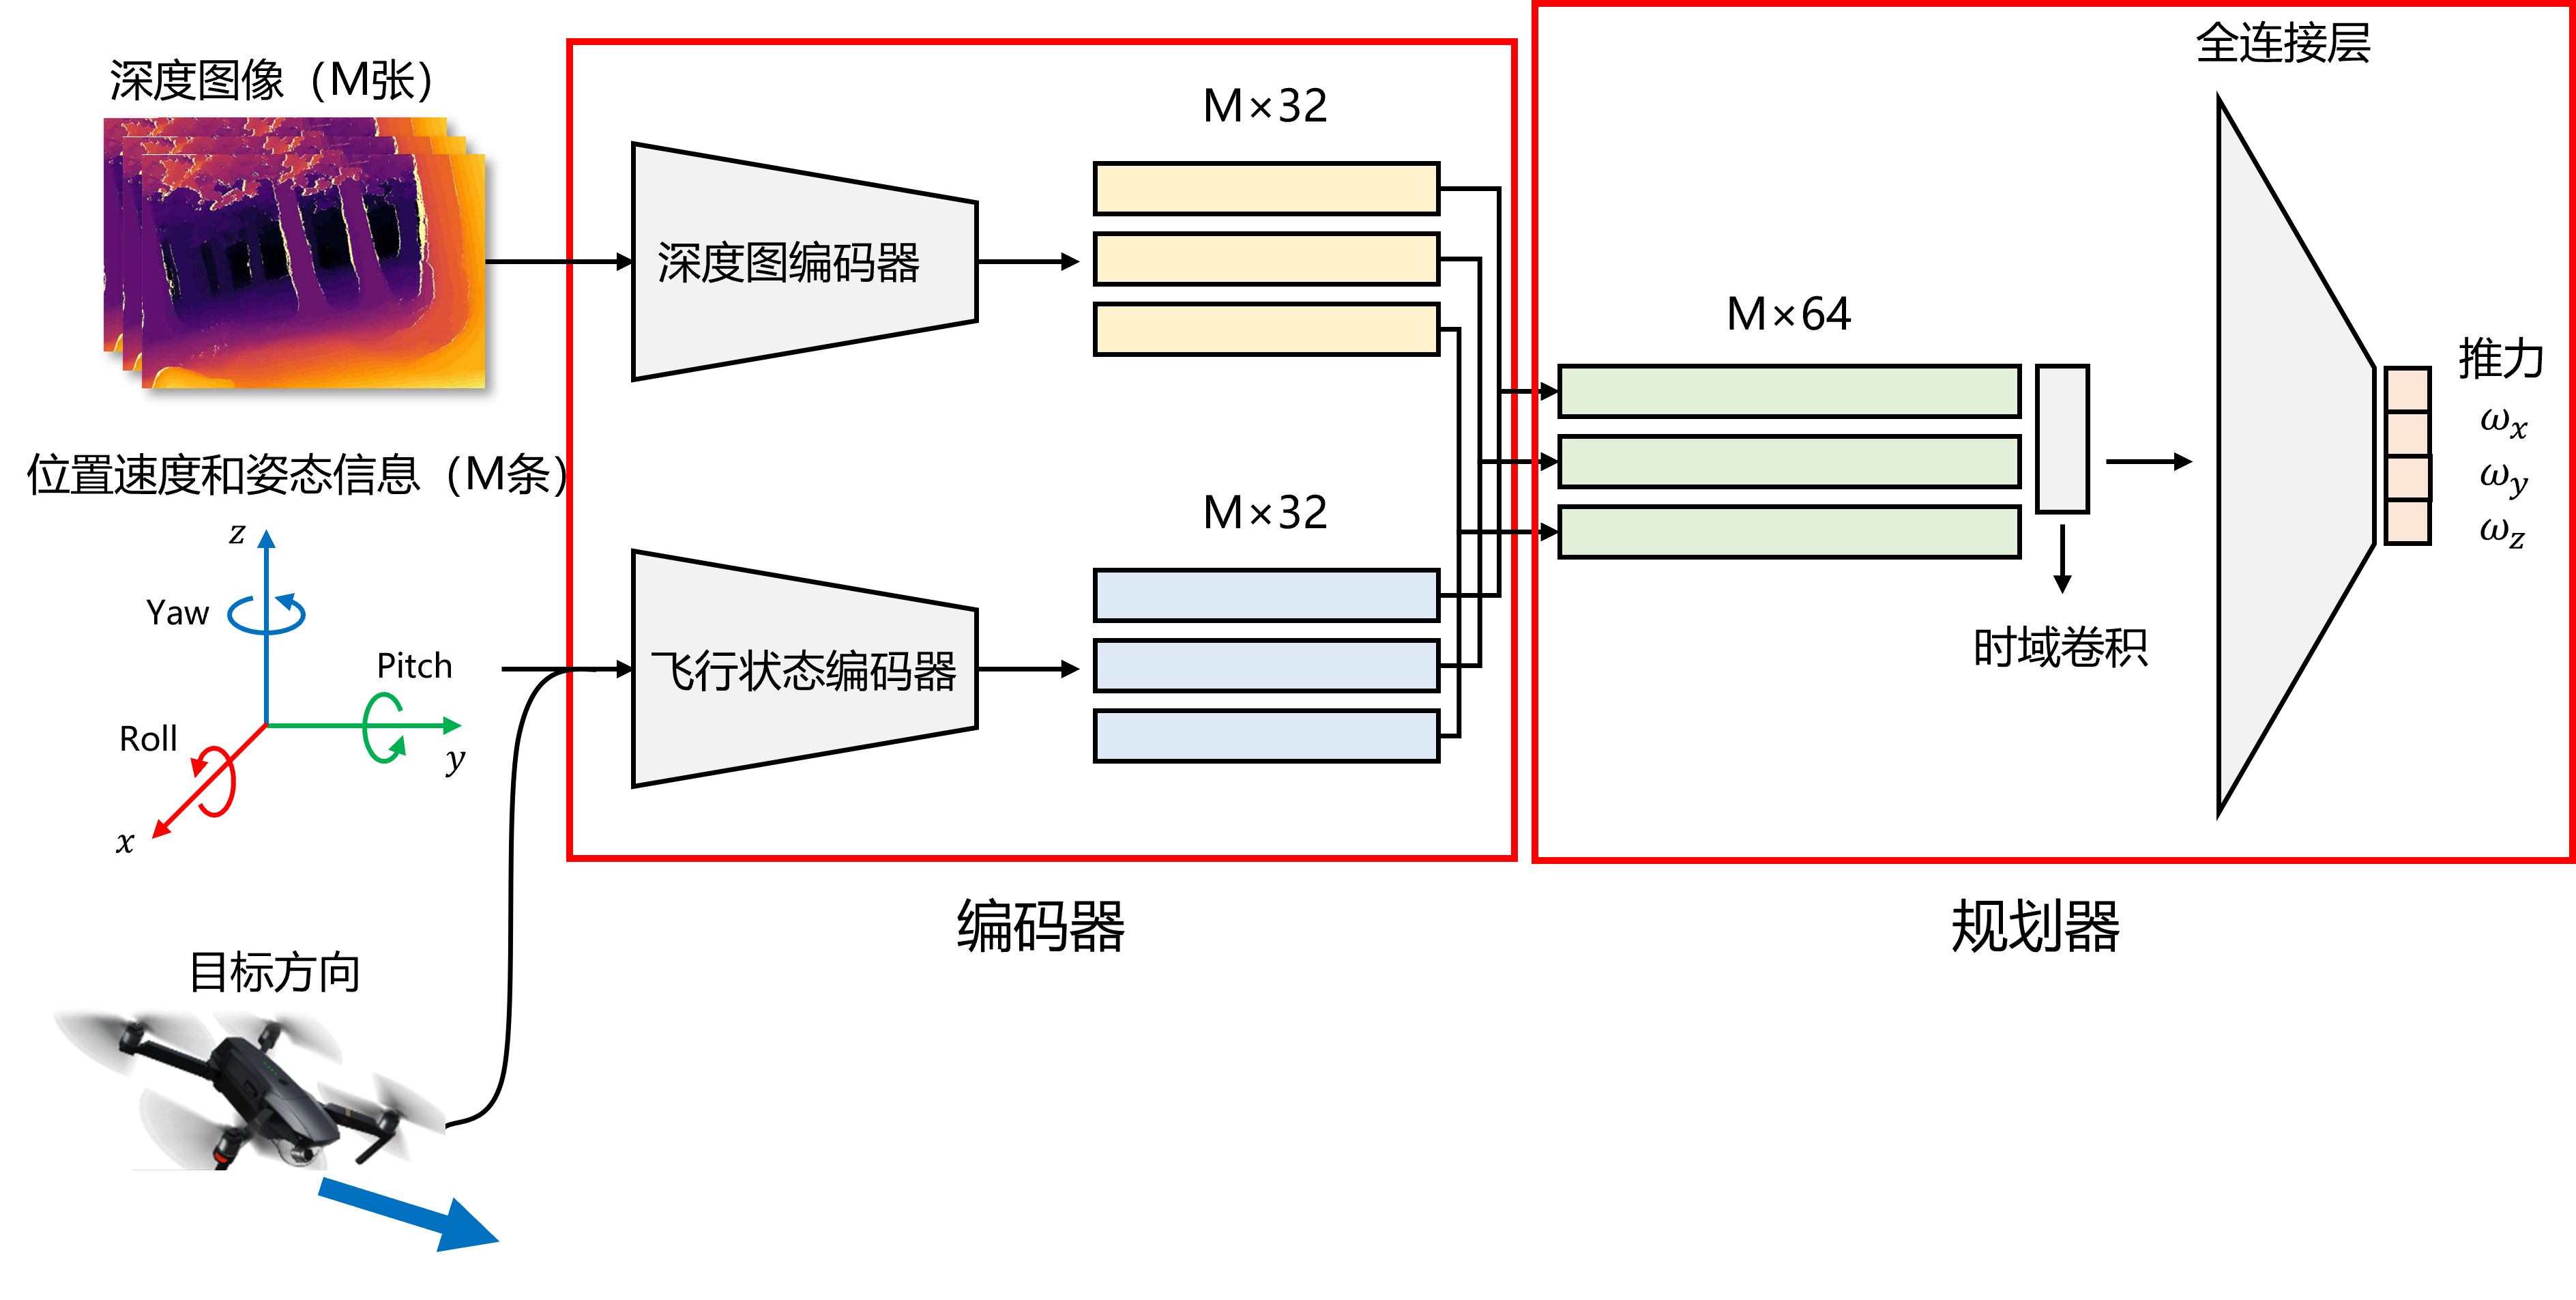
\includegraphics[width = 1\textwidth]{framework.png}
  \caption{自主导航端到端算法框架}
  \label{fig_framework}
\end{figure}

\subsection{输入和输出}
正如\ref{related_works}节所讲,无人机自主飞行任务常被划分为感知、决策、控制三部分,但实践中这样的划分往往并不绝对。为加快计算速度,本框架采用端到端的方式,将决策和部分感知、控制算法融合。框架的输入包括由IMU测量的无人机速度、加速度、角速度、角加速度;由深度相机得到的深度图,分辨率为$320\times240$像素;以及由视觉里程计(Visual-inertial odometry, VIO)输出的飞行器位置与角位置。特别地为增强算法稳定性,算法实际输入为过去一段时间的输入序列,实践中取这段序列长度为3,即$t$时刻的输入为$t-1,\ t-2,\ t-3$时刻的深度图和飞行器位置、速度、加速度信息。

企图控制一台飞行器,算法的输出也是多样的,例如飞行器的线速度和角速度、飞行器的总推力(Collective thrust)和角速度、飞行器四个旋翼的推力或转速等。相关工作表明\cite{kaufmann2022benchmark}输出为总推力与角速度(Collective thrust and body rates, CTBR)的策略往往会产生更稳健的效果,在仿真器和现实世界中的动力学差异也更小且该命令更具可解释性。因此本框架的输出为CTBR命令。在输出CTBR指令后,由飞行控制器将CTBR指令转换为四个电动机推力并执行。

\subsection{编码器(Encoder)}
\label{encoder}
无人机的输入是多模态(Multimodal)的,即包含可表达为21维向量的飞行器状态信息和可表达为320*240矩阵的深度图像,算法输入具体情况见表\ref{tab_input}。这些信息直接输入规划器可能会引起以下两个问题:
\begin{enumerate}
  \item 维度爆炸。深度图像素数量为$320\times240=76800$,维度过高,训练难度大,难以收敛。
  \item 信息不对称。深度图和飞行器状态两条输入的维度差距过大,可能会导致算法过于关注某一条输入,而忽略另一条输入。
\end{enumerate}
因此在正式输入规划器前需要两个编码器将输入信息编码为统一的维度和格式。两个编码器的结构如图\ref{fig_dep_encoder}, \ref{fig_state_encoder}中编码器部分所示。飞行状态编码器主要由时域卷积模块(Temporal Convolutional)组成,将飞行器状态信息编码时域卷积为$3*32$维。深度图编码器先经过一个MobileNetV3\cite{Howard_2019_ICCV}编码为512维向量,再通过一个时域卷积模块同样编码为$3*32$维。
\begin{table}
  \centering
  \begin{tabular}{ccccc}
  \hline
  \textbf{输入来源} & VIO & IMU & 深度相机 & 任务目标\\ \hline
  \textbf{输入形状} & 12维向量 & 6维向量 & 320*240矩阵 & 3维向量\\ \hline
      \multirow{2}*{\textbf{输入描述}} & 无人机位置3维 & \multirow{2}*{线速度与角速度} & \multirow{2}*{深度图像}  & \multirow{2}*{指向目标的单位向量}\\ 
      & 姿态旋转矩阵9维 & & \\ \hline
  \end{tabular}
  \caption{自主导航算法输入}
  \label{tab_input}
\end{table}

\begin{figure}
  \centering
  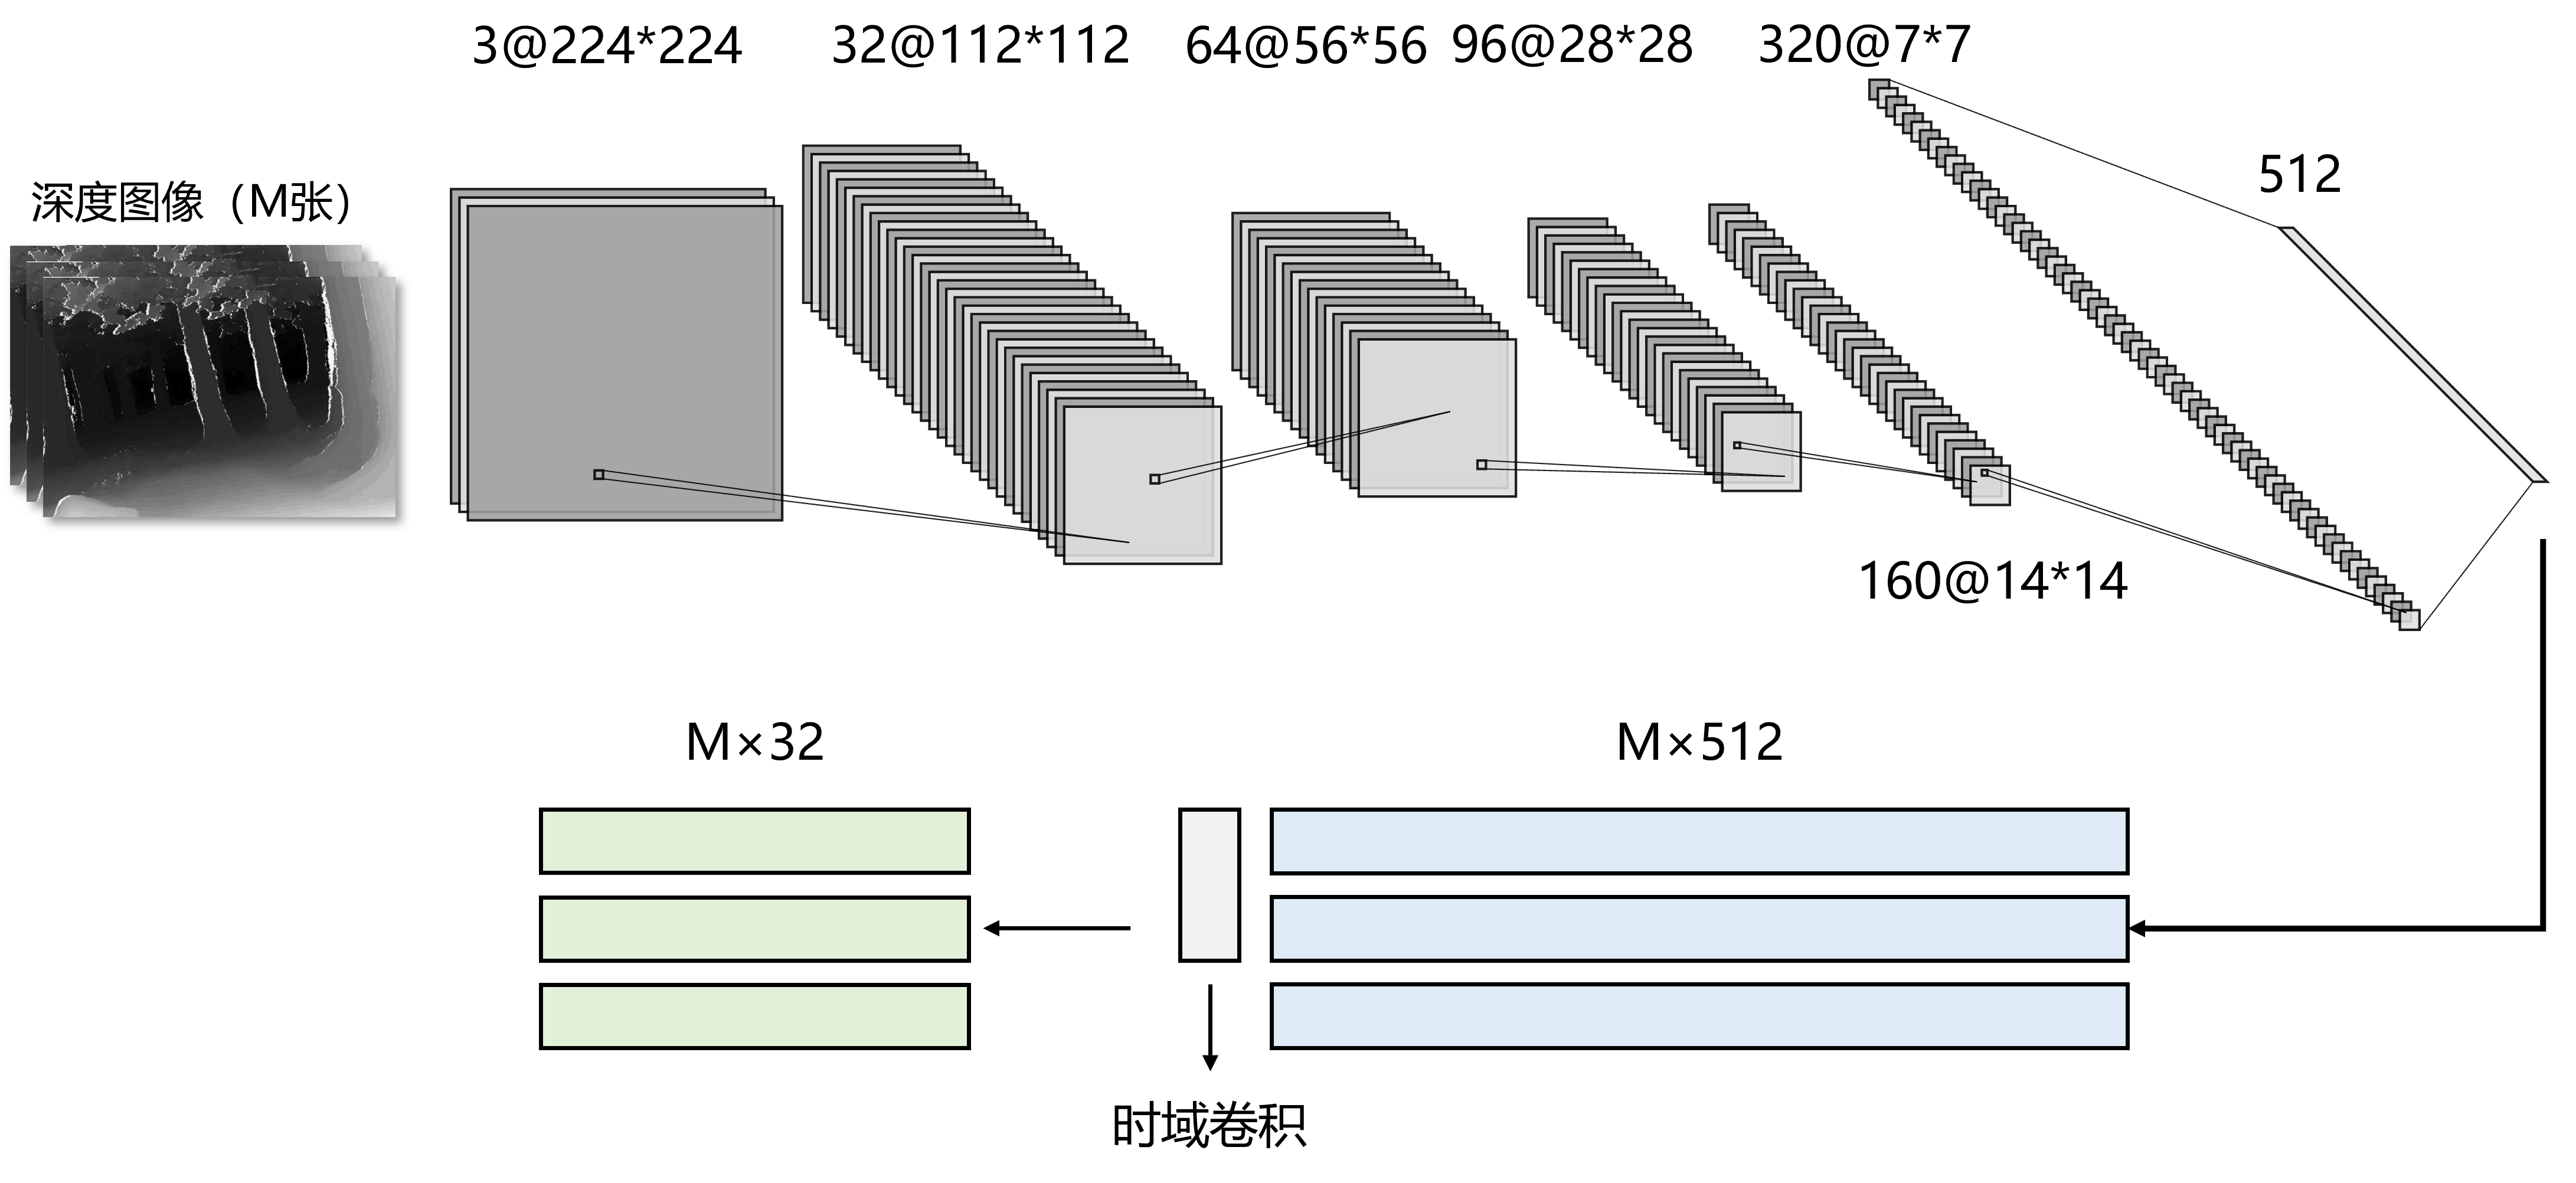
\includegraphics[width = 1\textwidth]{dep_encoder.png}
  \caption{深度图编码器结构图}
  \label{fig_dep_encoder}
\end{figure}

\begin{figure}
  \centering
  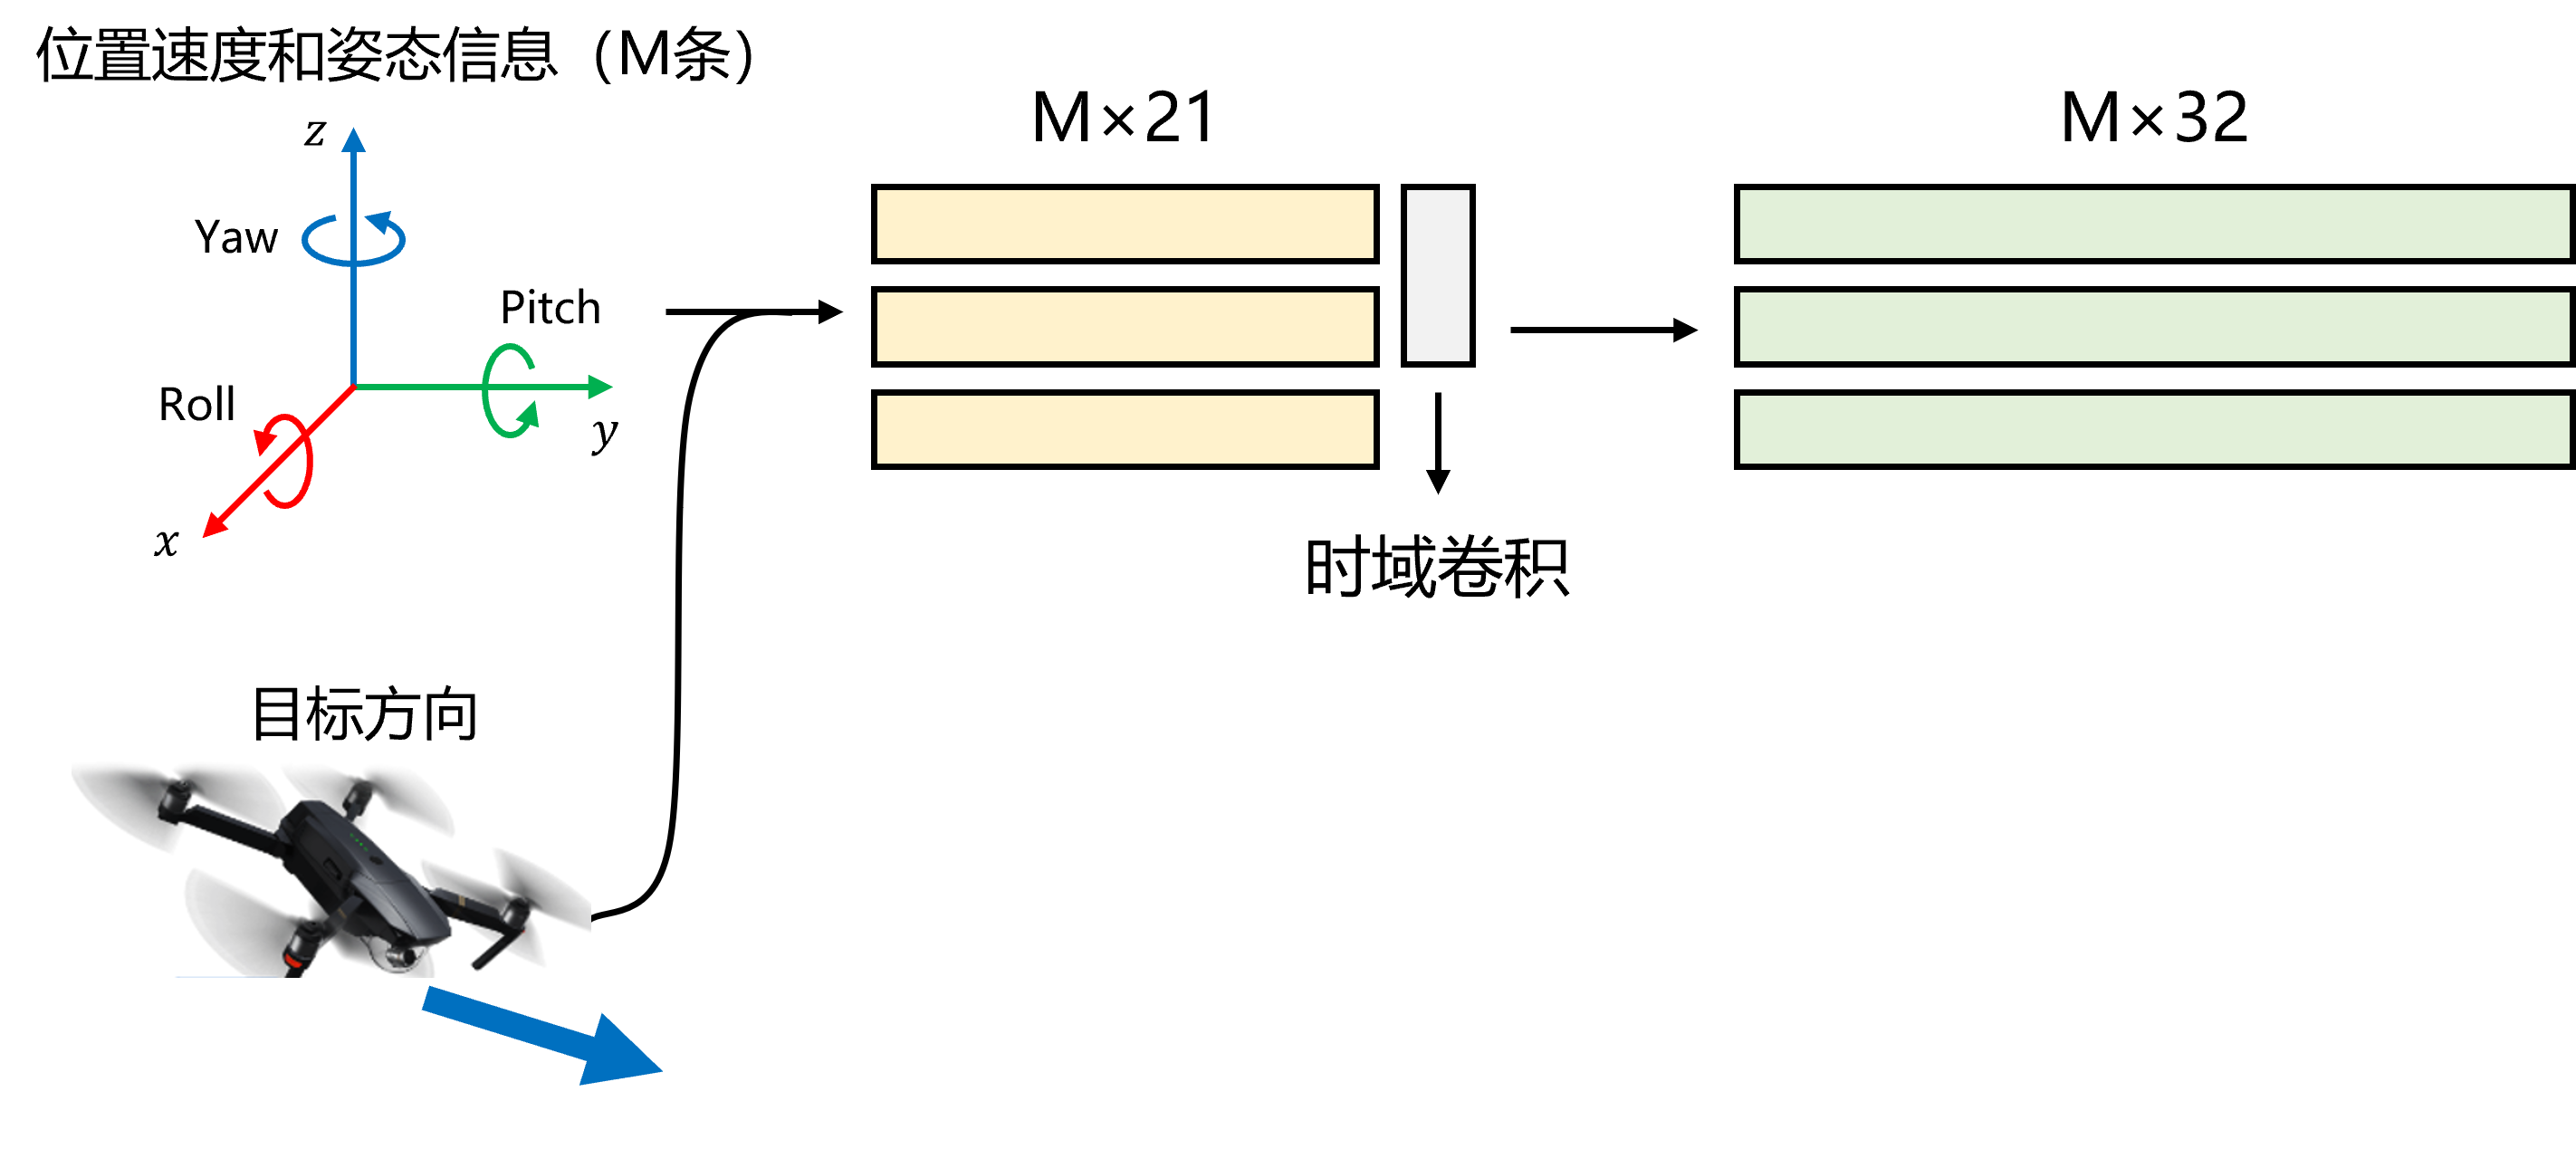
\includegraphics[width = 0.8\textwidth]{state_encoder.png}
  \caption{飞行状态编码器结构图}
  \label{fig_state_encoder}
\end{figure}

\subsection{规划器(Planner)}
将编码器编码过的两个$3*32$维的矩阵拼接为$3*64$维的矩阵,作为规划器的输入。规划器的结构如图\ref{fig_planner}所示,由一个时域卷积模块和一个全连接层组成。在时域再次进行卷积后输入全连接层,经过$[512, 256, 128, 64]$节点的四个隐藏层后输出为$4$维,分别表示CTBR四个维度的指令。规划器的输出会被送入飞行控制器,由飞行控制器将CTBR指令转换为四个电动机推力并执行。
\begin{figure}
  \centering
  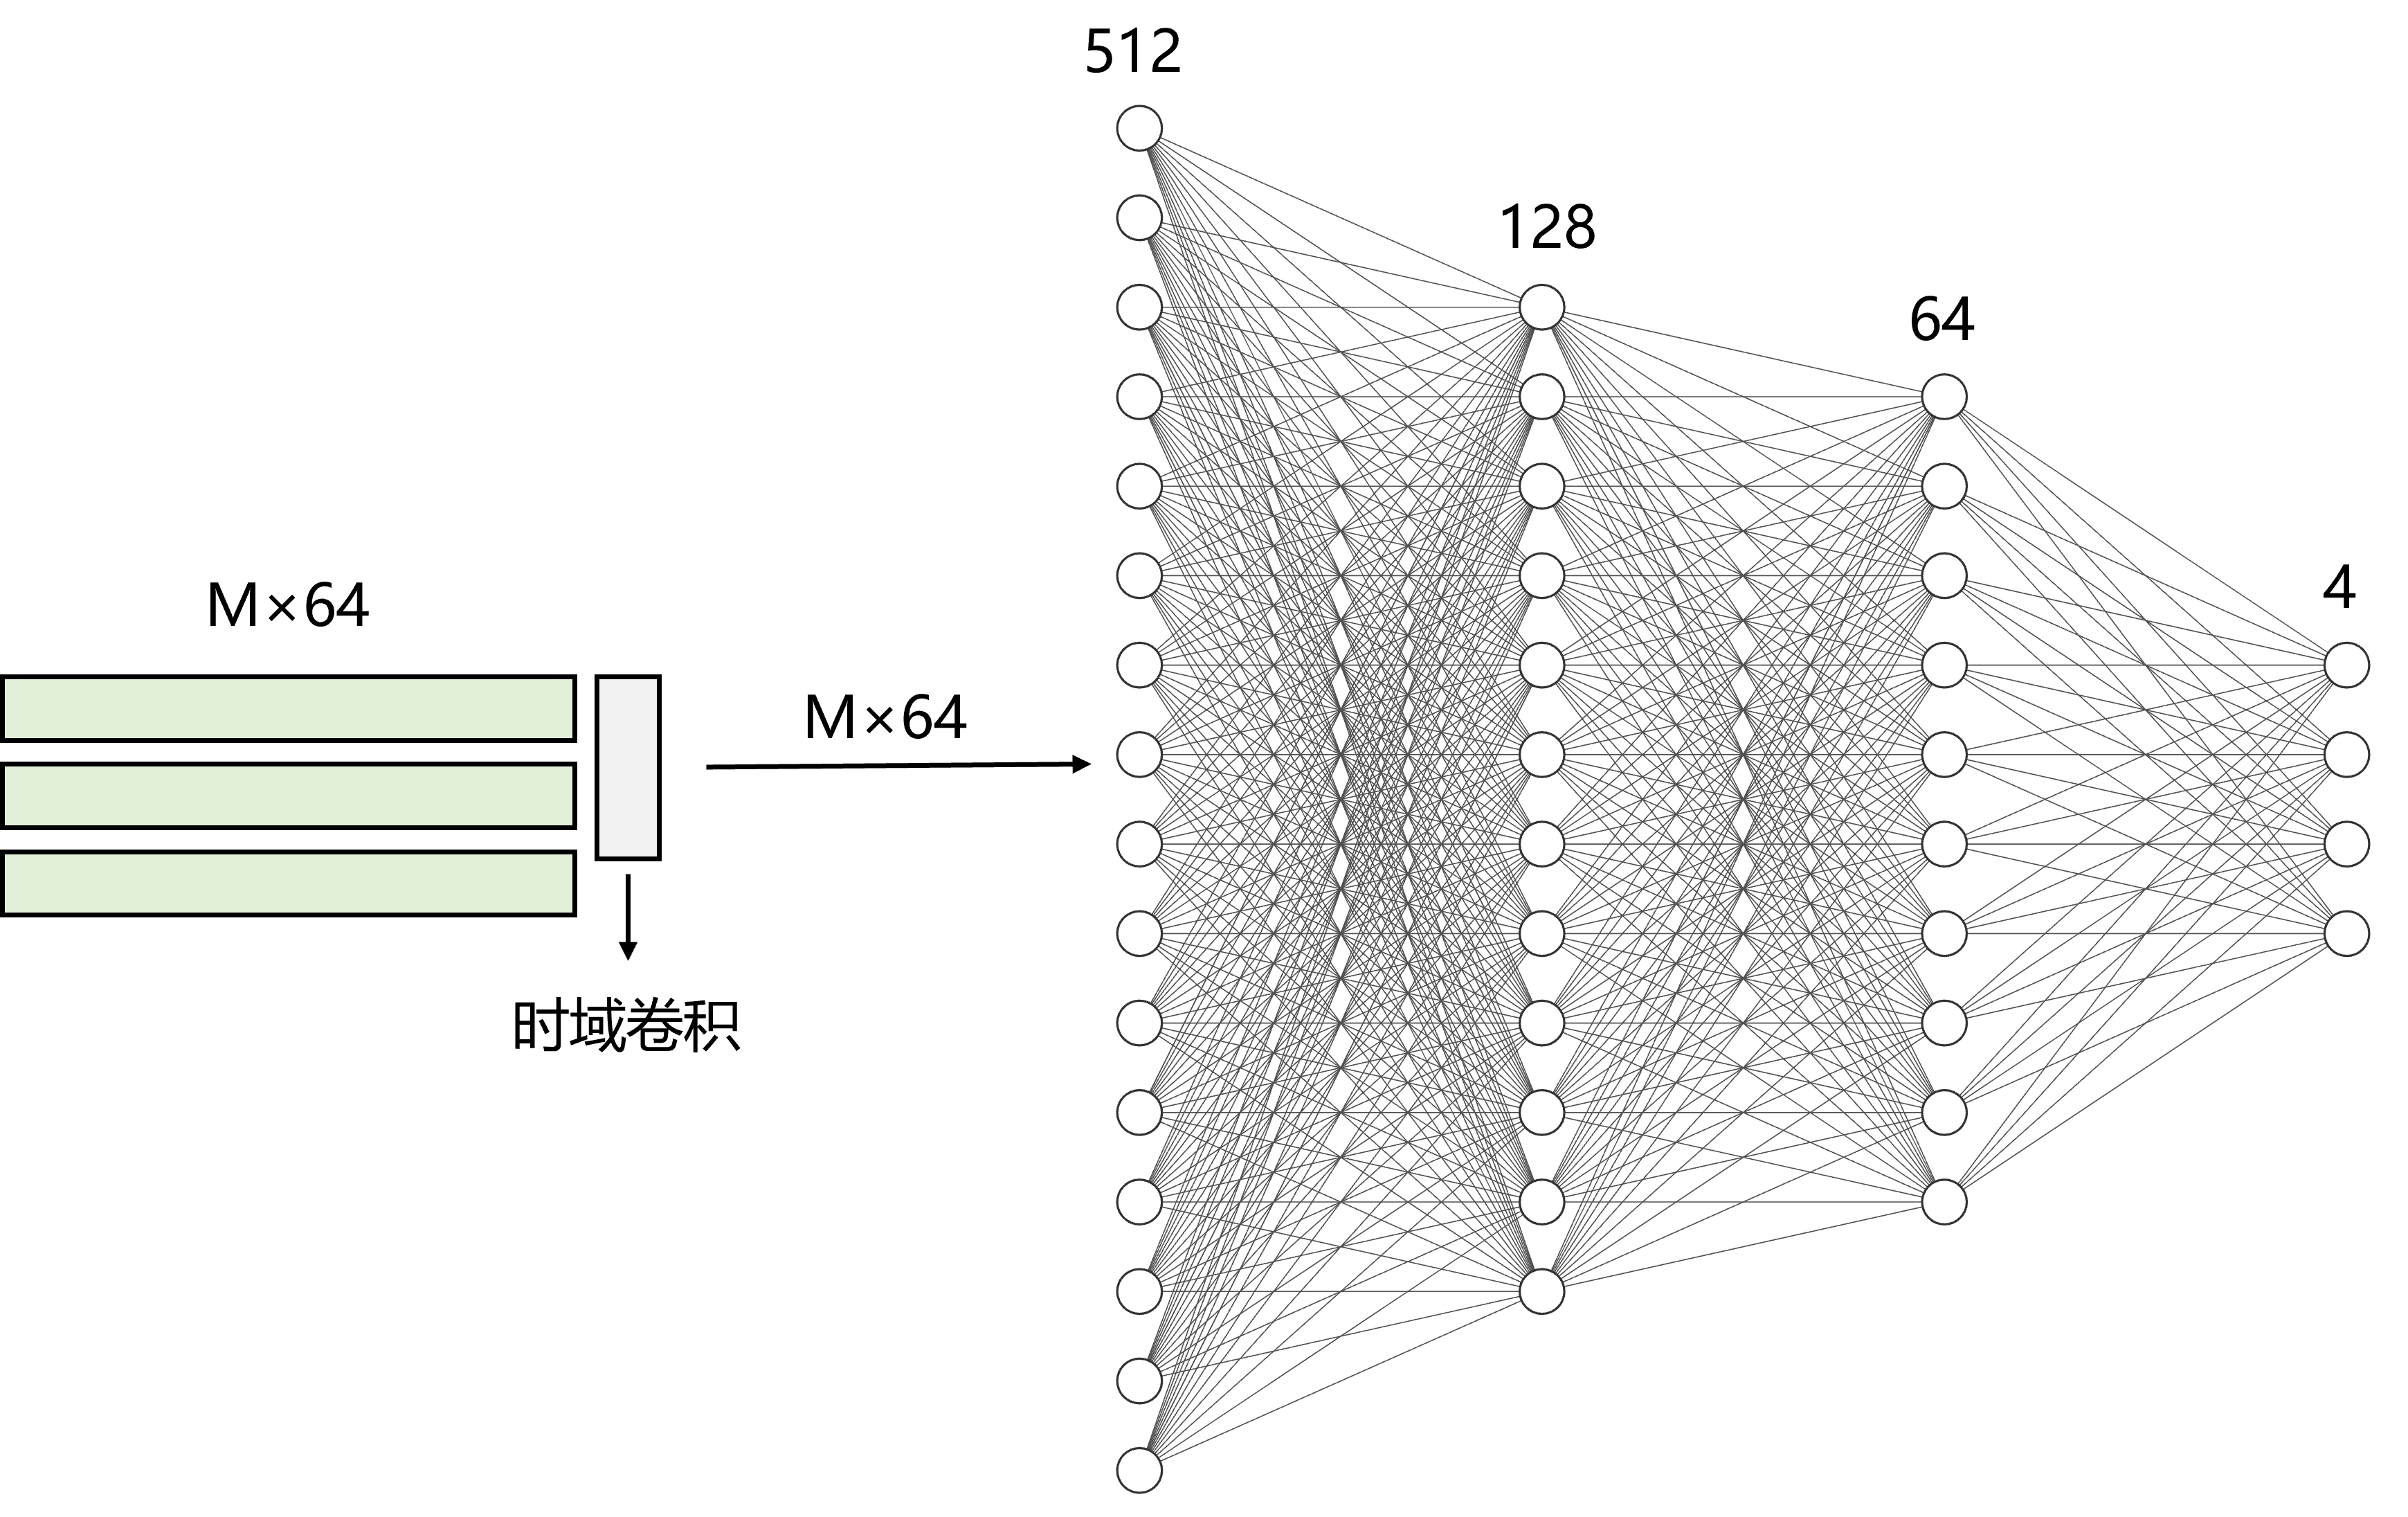
\includegraphics[width = 0.9\textwidth]{planner.png}
  \caption{规划器结构图}
  \label{fig_planner}
\end{figure}
经过实验与调研\cite{loquercio2021learning},该端到端框架相比传统感知-建图-规划的方法执行速度更快,与其它基于学习的方法执行速度类似,测试结果如表\ref{tab_exetime}所示。

\begin{table}
  \centering
  \begin{tabular}{ccccc}
  \hline
      \textbf{方法} & \textbf{阶段} & \textbf{用时(ms)} & \textbf{占比} & \textbf{总用时} \\ \hline
      \multirow{3}*{FastPlanner\cite{zhou2019robust}} & 预处理 & 14.6 & 22.4\% & \multirow{3}*{65.2} \\ %\cline{2-4}
      ~ & 建图 & 49.2 & 75.5\% & ~ \\ %\cline{2-4}
      ~ & 规划 & 1.4 & 2.1\% & ~ \\ \hline
      \multirow{2}*{Reactive\cite{florence2020integrated}} & 预处理 & 13.8 & 72.3\% & \multirow{2}*{19.1} \\ %\cline{2-4}
      ~ & 规划 & 5.3 & 27.7\% & ~ \\ \hline
      \multirow{3}*{Learning Planner\cite{loquercio2021learning}} & 预处理 & 0.1 & 1\% & \multirow{3}*{10.3} \\ 
      ~ & 神经网络推理 & 10.1 & 98\% & ~ \\ 
      ~ & 规划 & 0.08 & 1\% & ~ \\ \hline
      \multirow{2}*{本方法} & 预处理 & 0.1 & 1\% & \multirow{2}*{13.3} \\ 
      ~ & 神经网络推理 & 13.2 & 99\% & ~ \\ \hline
  \end{tabular}
  \caption{各自主导航算法执行时间}
  \caption*{测试平台为Intel Core i7-8700K CPU, NVIDIA GeForce RTX 2080 GPU}
  \label{tab_exetime}
\end{table}

\section{训练方法}
\subsection{三段式训练方法}
将自主导航算法整体接入仿真器训练,经测试训练各模块运行频率如表\ref{train_freq}所示。Unity渲染深度图像运行频率慢,成为训练瓶颈。为此本研究提出了三段式训练方法,主要思路是在在线(Online)强化学习阶段使用更快速获取的信息(点云)作为输入以避免渲染深度图像对训练速度的影响。具体地,三段式训练方法如图\ref{fig_step1},\ref{fig_step2},\ref{fig_step3}所示。第一阶段需在采集好的点云数据集上使用自动编码器 (Autoencoder)的方法训练点云编码器。第二阶段将预训练的点云编码器和点云输入接入规划器,进行在线强化学习训练。第三阶段再采集点云-深度图像数据对,有监督地训练深度图编码器。在部署时仅需要接入分别在第二、三步训练好的深度图编码器和规划器即可。下面将分别详细介绍这三个步骤。
\begin{table}
  \centering
  \begin{tabular}{ccccc}
      \hline
      \textbf{仿真模块} & \textbf{Unity渲染深度图} & \textbf{Gazebo动力学模拟} & \textbf{控制器} & \textbf{神经网络推理} \\ \hline
      运行频率(Hz) & 15$\sim$30 & 2000 & $>$1000 & $>$300 \\ \hline
  \end{tabular}
  \caption{仿真器各模块运行频率}
  \caption*{测试平台为Intel Core i9-13900K CPU, NVIDIA GeForce RTX 4090 GPU}
  \label{train_freq}
\end{table}

\begin{figure}
  \centering
  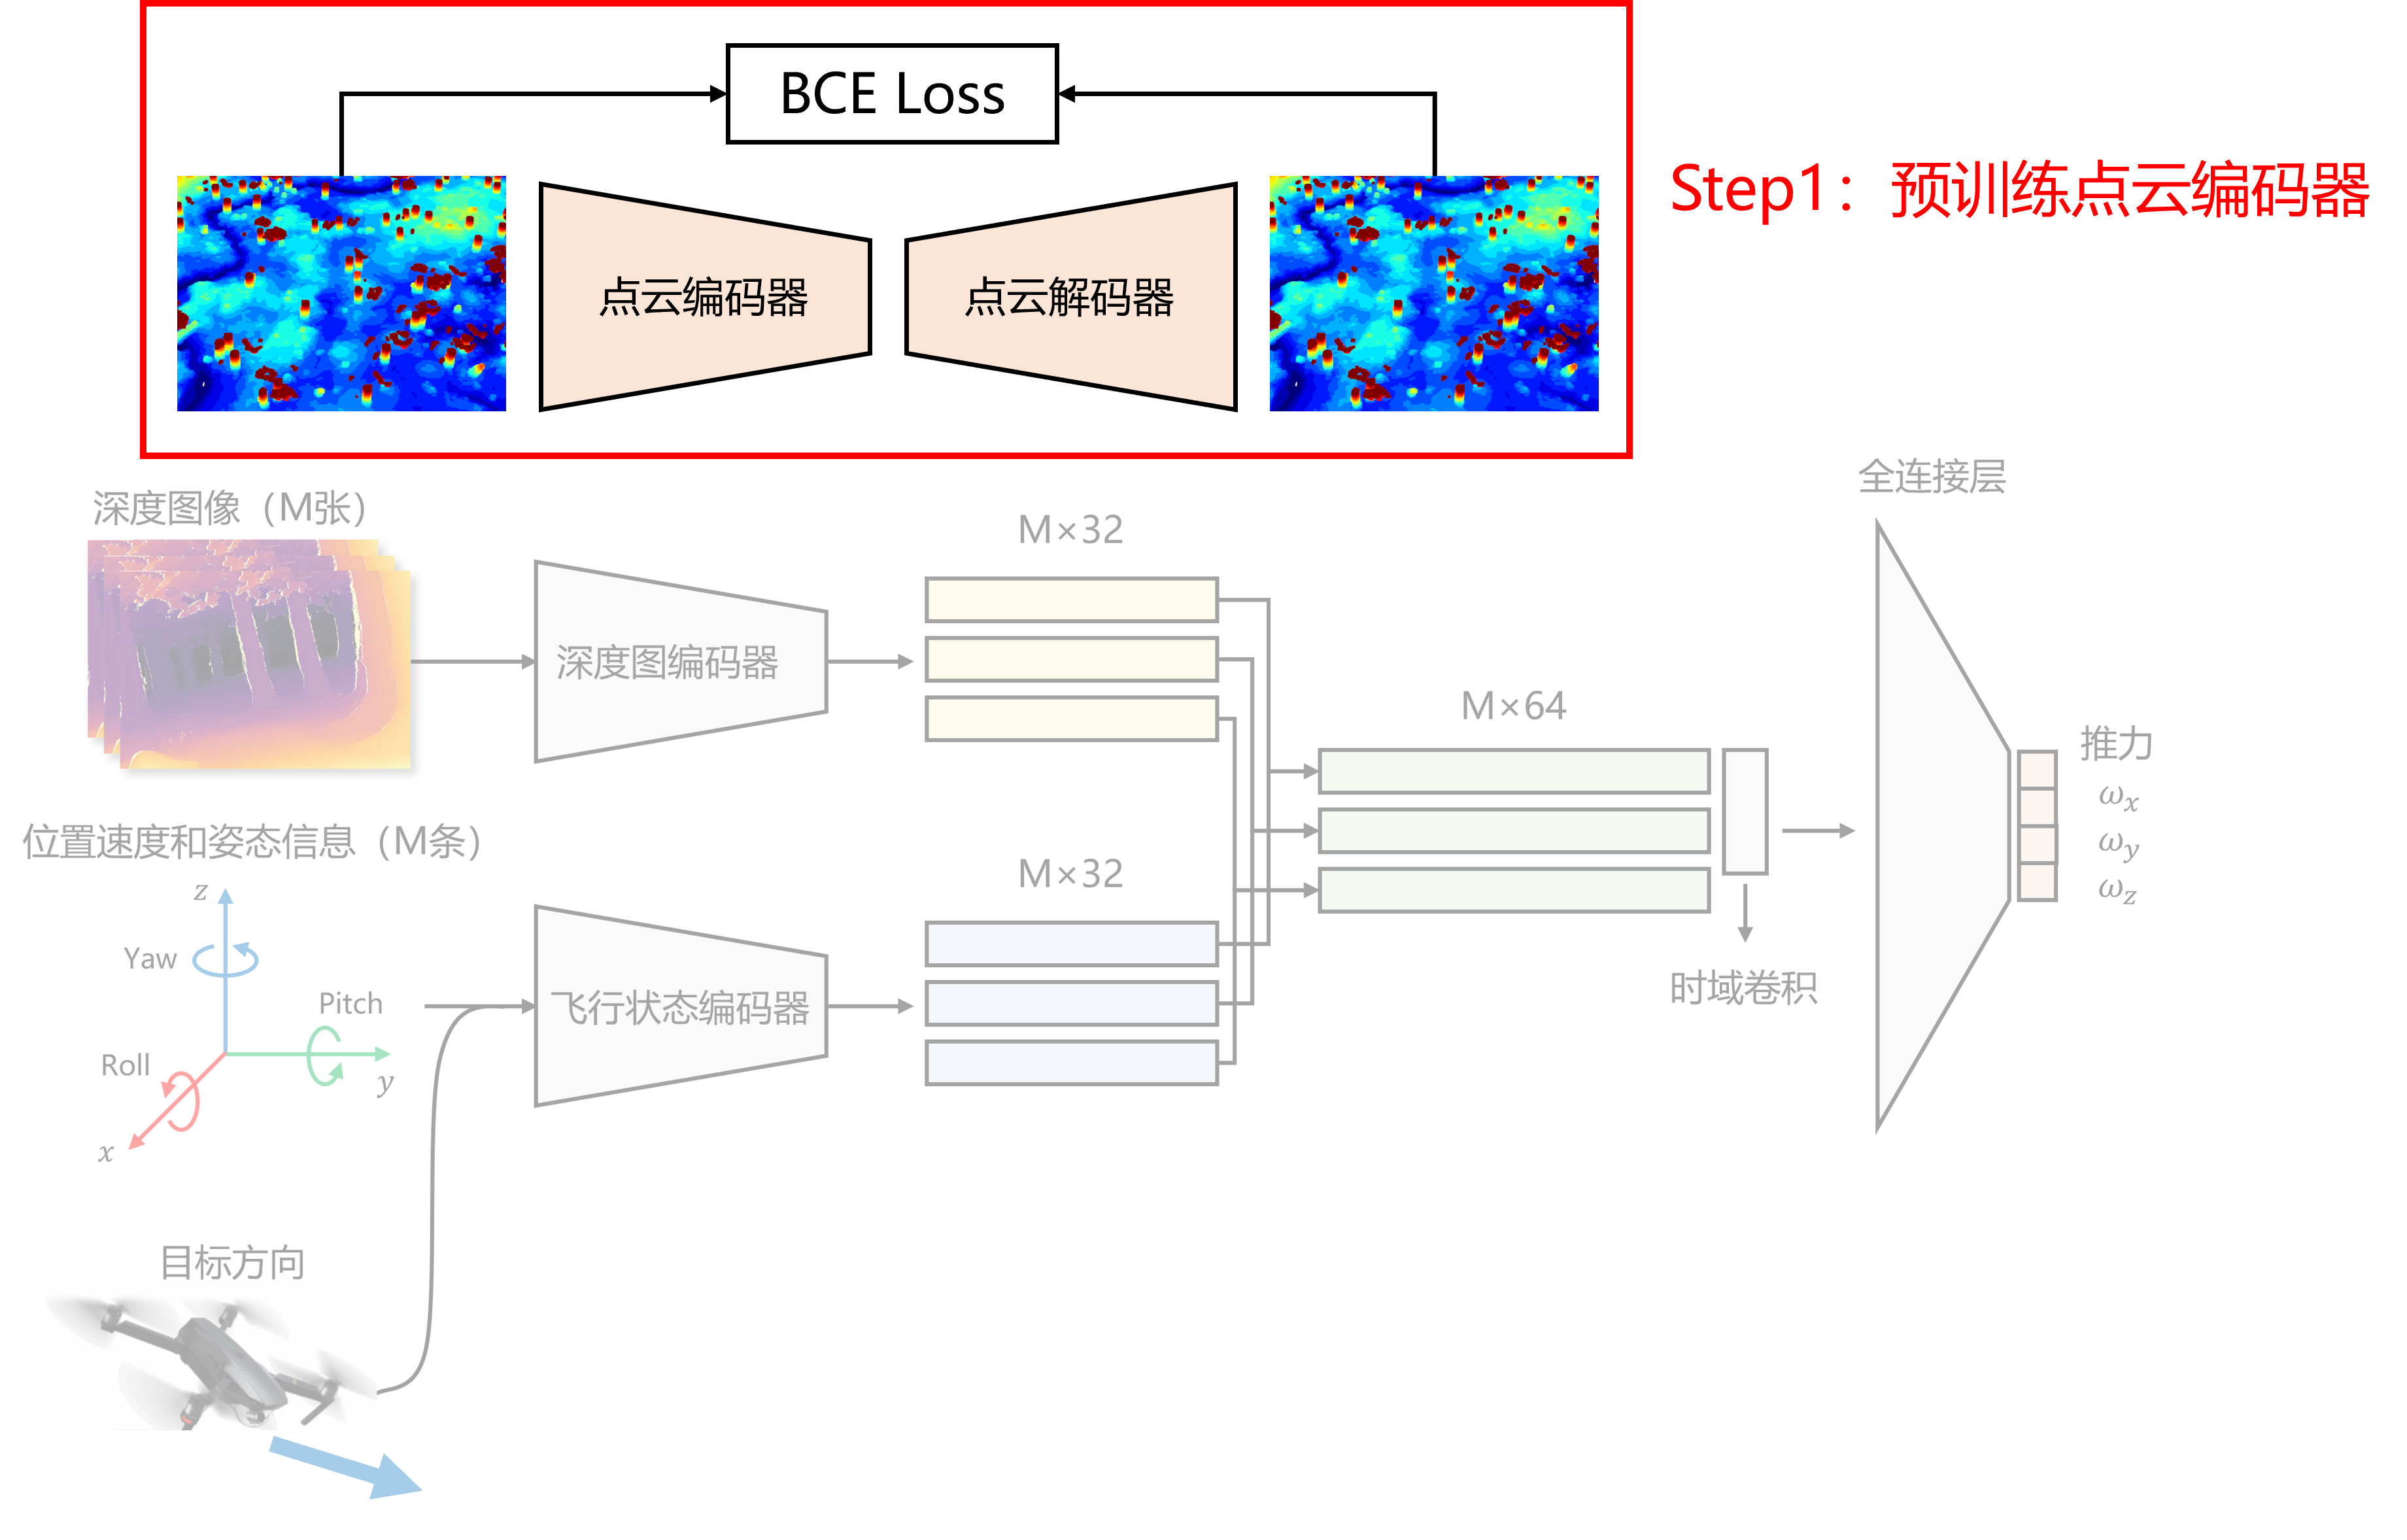
\includegraphics[width = 0.95\textwidth]{step1.png}
  \caption{预训练点云编码器}
  \label{fig_step1}
\end{figure}

\begin{figure}
  \centering
  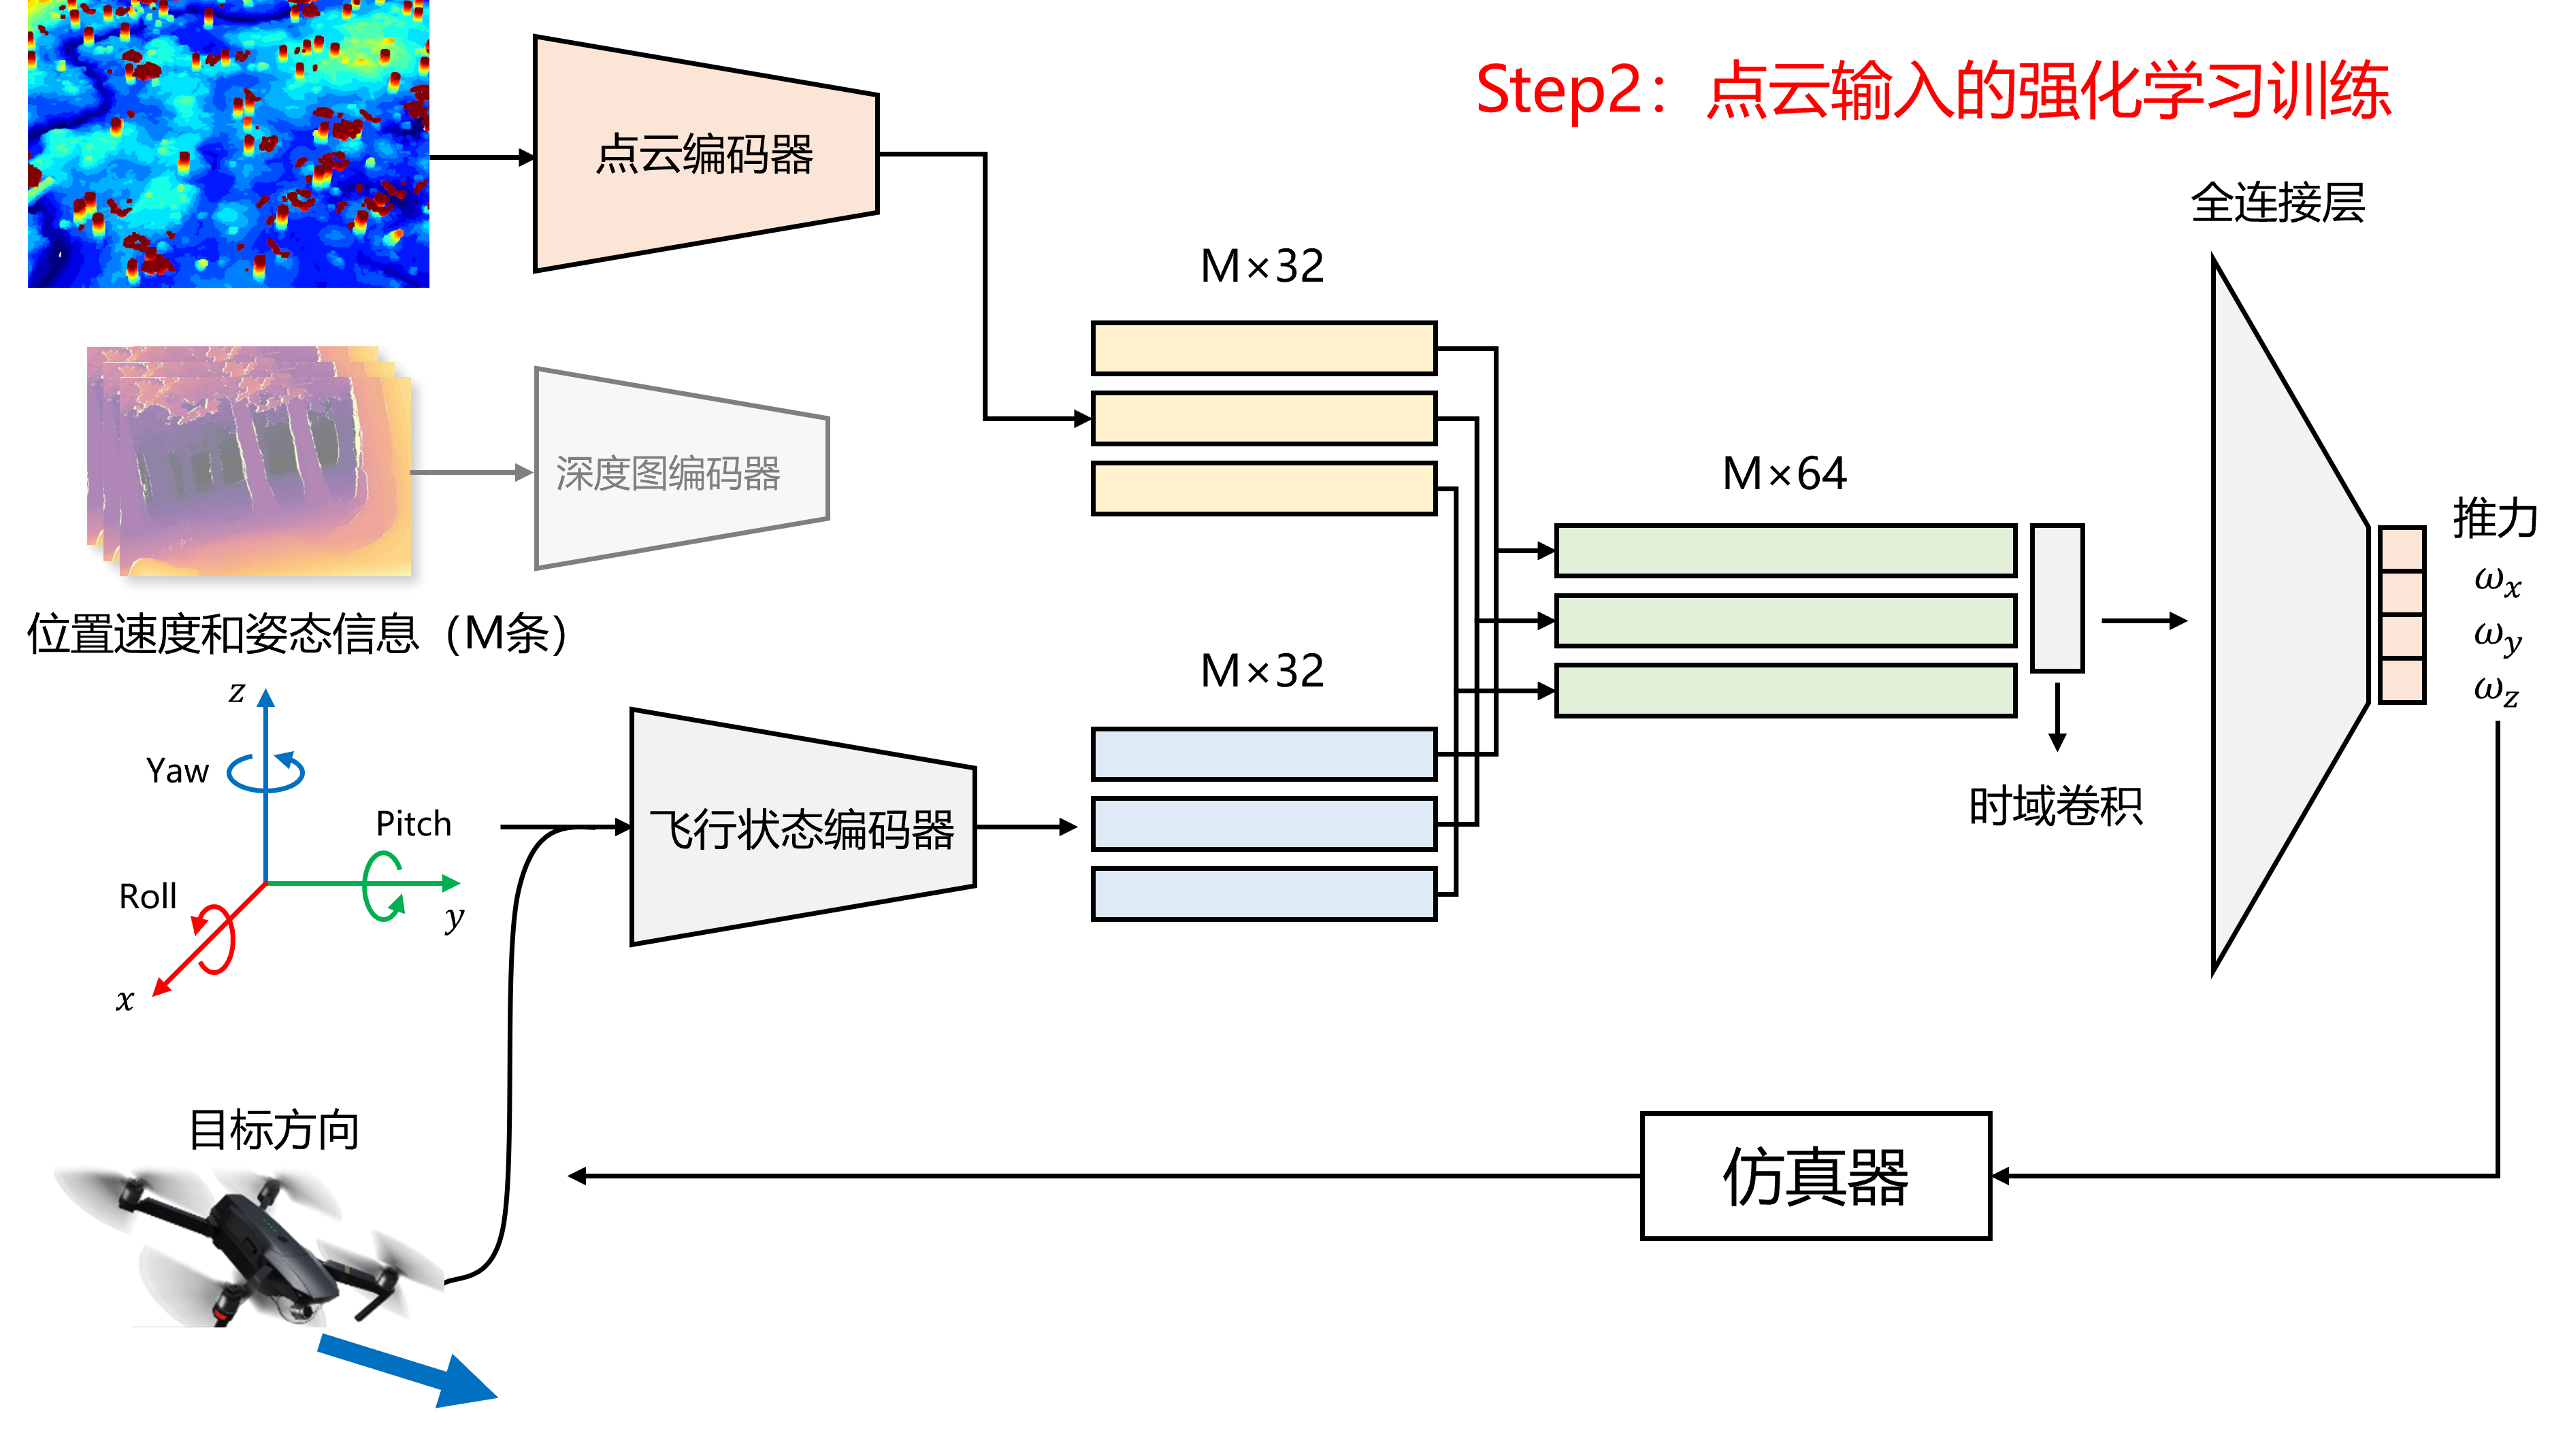
\includegraphics[width = 1\textwidth]{step2.png}
  \caption{点云输入的强化学习训练}
  \label{fig_step2}
\end{figure}

\begin{figure}
  \centering
  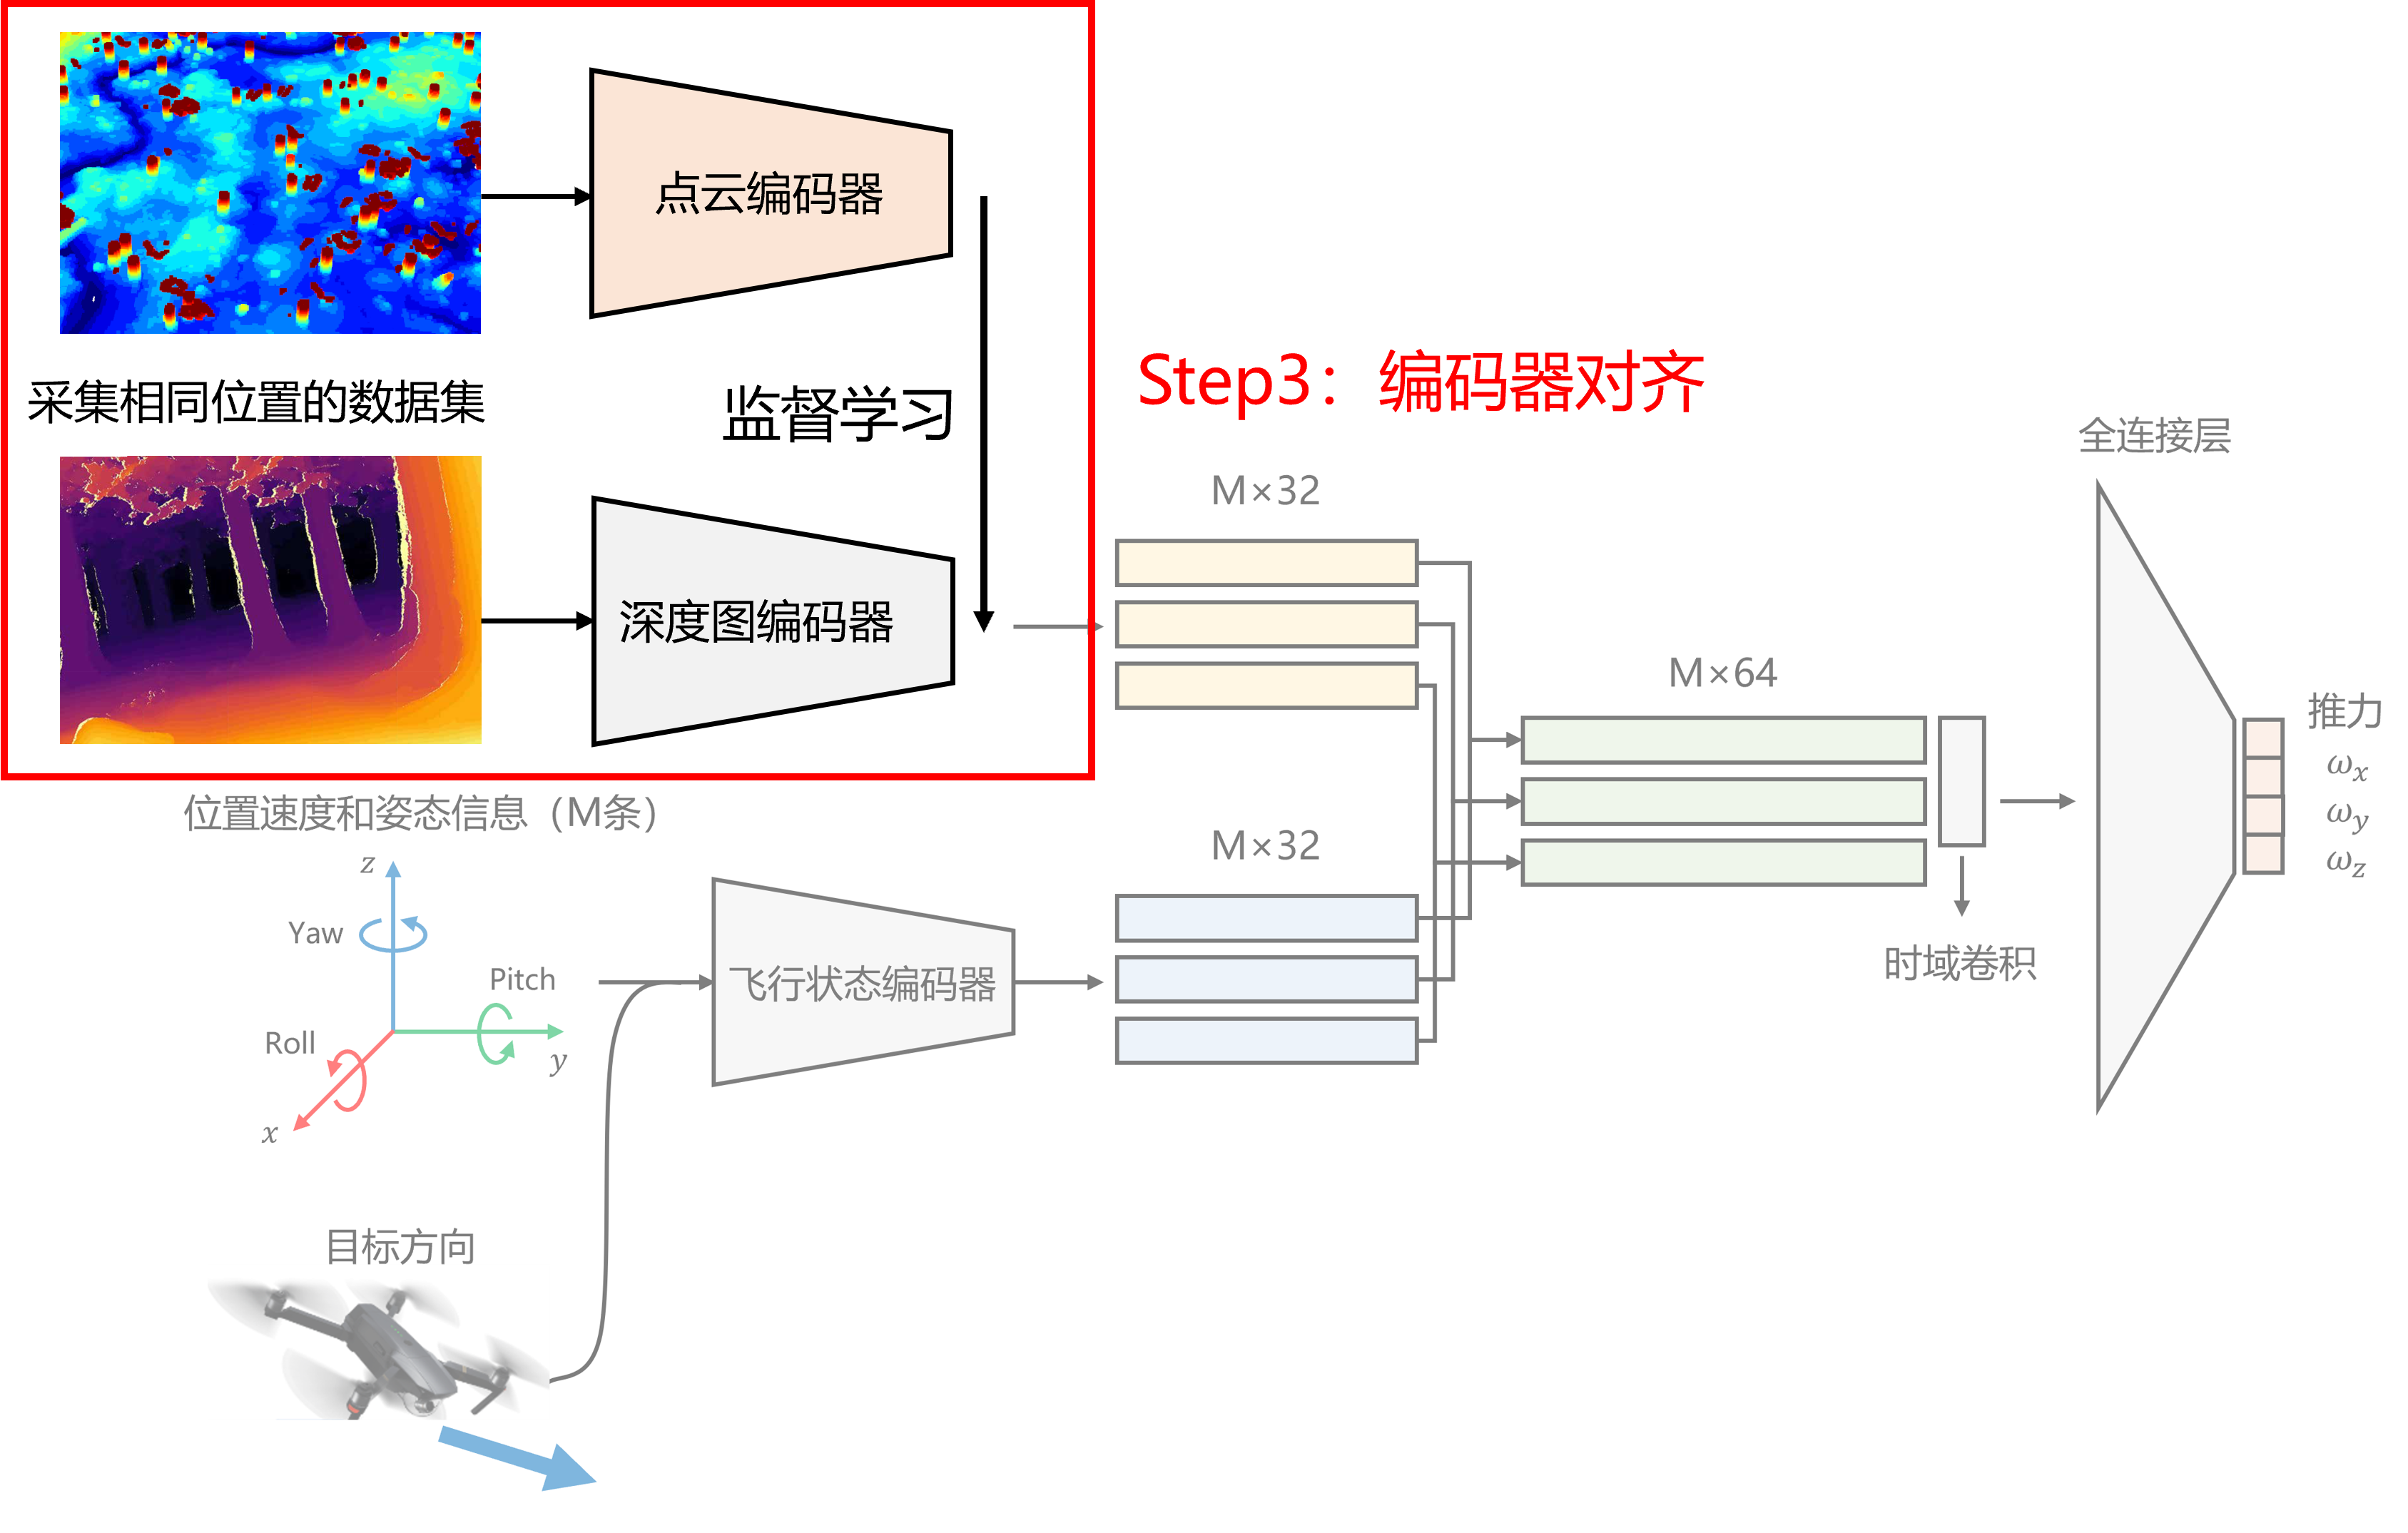
\includegraphics[width = 0.89\textwidth]{step3.png}
  \caption{编码器对齐}
  \label{fig_step3}
\end{figure}

\subsubsection{预训练点云编码器}
\label{pcd_encoder}
同\ref{encoder}节所讲,以点云为输入的训练同样需要点云编码器。虽然无人机自主导航任务的环境是未知的,但环境的类型和大体分布是已知的。我们预渲染了几百幅地图的点云数据,从中随机裁剪(Crop)大小与深度相机感知范围一致,即$3m\times 3m\times 2m$的点云块。这些随机采集的点云块数据集与飞行中可能遇到的点云输入是类似的,因此可以在点云块数据集上训练点云编码器,如图\ref{fig_step1}。点云编码器的结构如图\ref{fig_pcd_encoder}所示,在其后接入与编码器对应的解码器(Decoder)以重建输入点云块。训练使用二进制交叉熵(Binary cross entropy, BCE)损失函数,将解码器重建的点云块与原始点云块对比做自监督训练。训练完成后,点云编码器可以将点云块编码为512维的向量,该向量就可作为规划器的输入。

\begin{figure}
  \centering
  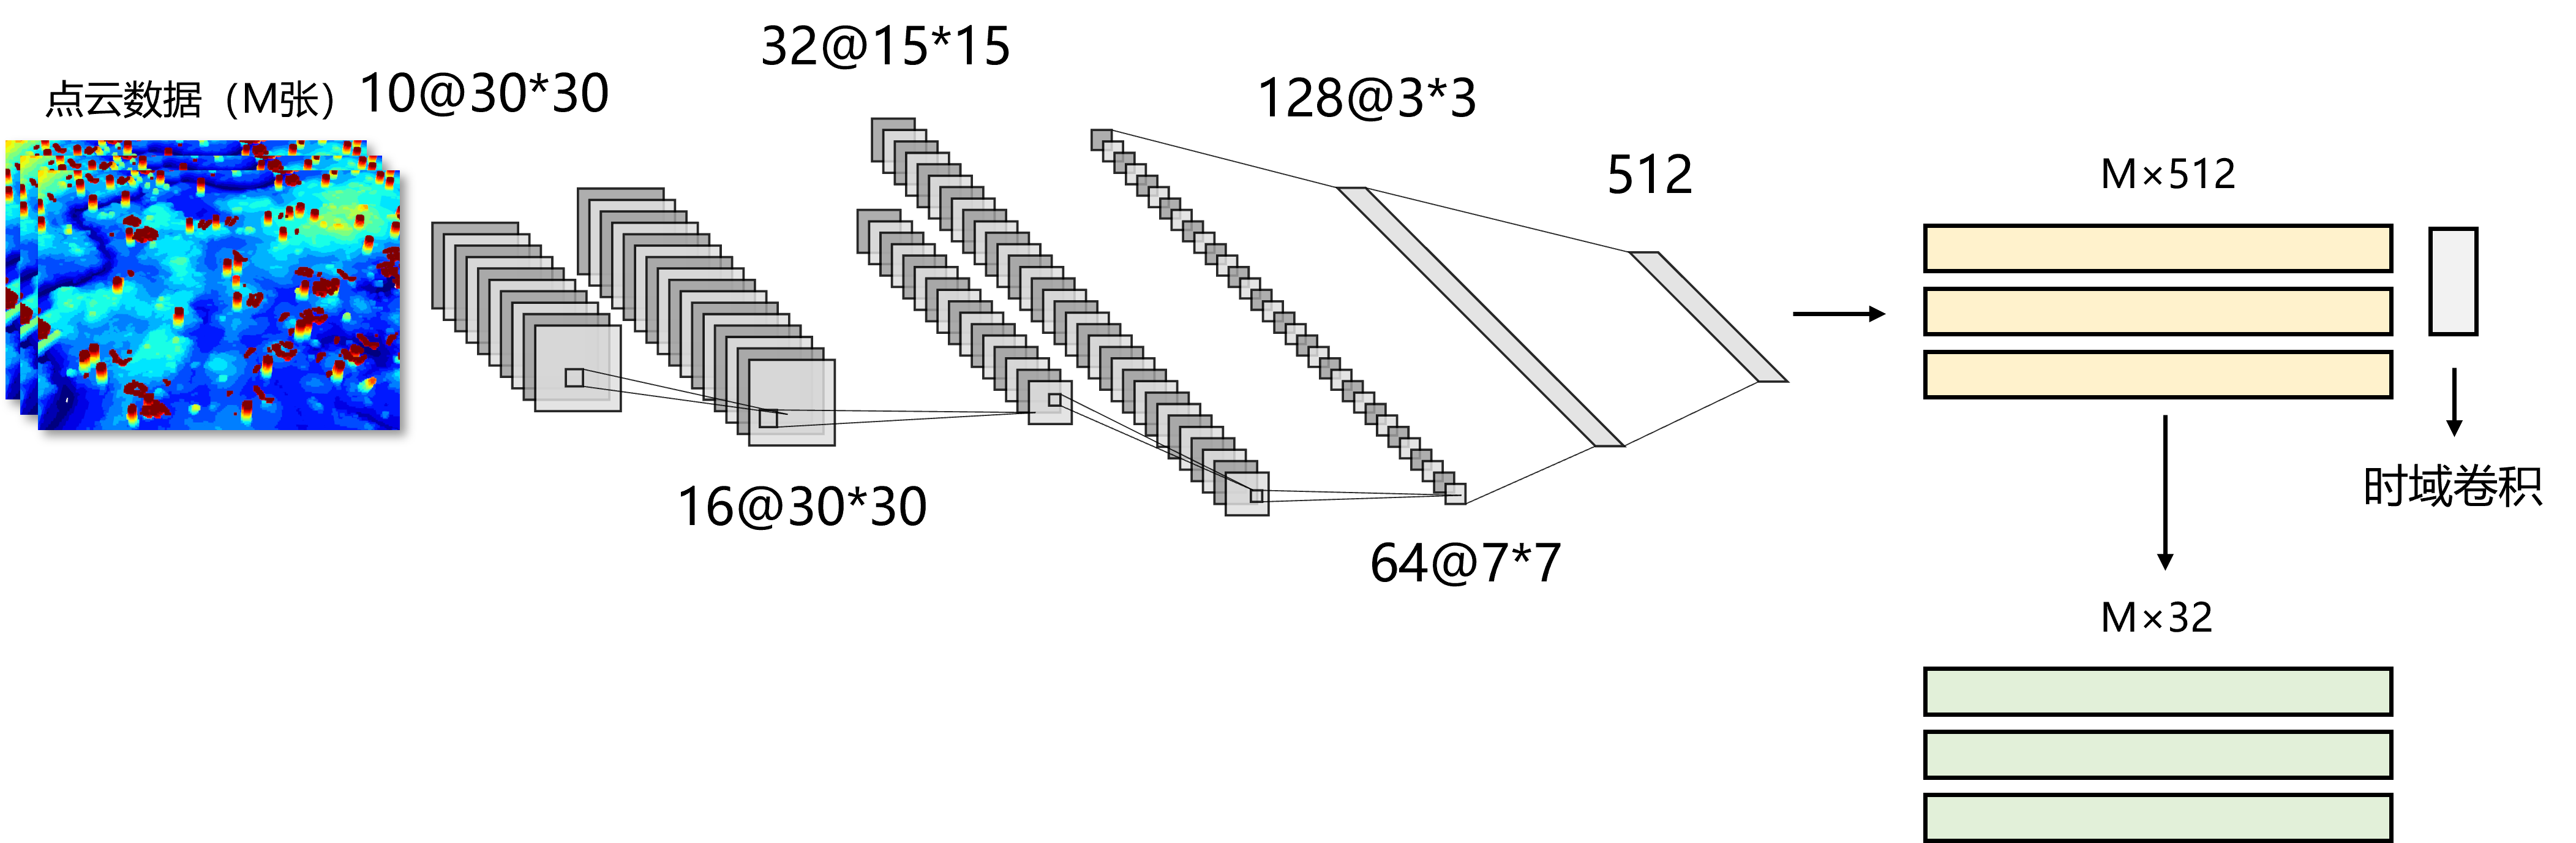
\includegraphics[width = 1\textwidth]{pcd_encoder.png}
  \caption{点云编码器结构图}
  \label{fig_pcd_encoder}
\end{figure}

\subsubsection{点云输入的强化学习训练}
\label{pcd_rl}
在获得点云编码器后,就可以使用使用点云编码器连接输入,用\ref{PPO_alg}节提到的PPO算法训练规划器。具体训练流程如图\ref{fig_step2}所示。训练中使用的奖励函数$\mathcal{R}$将在\ref{reward_design}节中详细介绍。在训练中为了进一步提高训练效率,还设计了以下两个技术细节:
\begin{enumerate}
  \item 编码器固定。强化学习的基本原理决定了其需要通过试错来改进策略。在训练最开始阶段,策略是几乎随机的。若编码器也被同时训练,可能会降低预训练编码器的性能。故在训练开始时先固定编码器参数,仅改变规划器使其能够在固定的编码器下学到较好的策略。当规划器训练到一定程度(具体表现为平均回合长度达到6s,即策略学会了基本的飞行)后,再开始以较低的更新率一同训练编码器,以微调其编码能力。
  \item 域随机化(Domain randomization)。在训练时将障碍物密度、起始位置、飞行参考速度等任务参数在一定比例范围内随机化,增加训练数据的多样性,提高模型的泛化能力。
\end{enumerate}

\subsubsection{编码器对齐}
\label{encoder_align}
使用点云作为输入是为了加速训练,而实际应用和部署的阶段仍需要深度相机拍摄的深度图作为输入。因此训练的最后一步就是以调整过后的点云编码器为监督,训练深度图编码器。我们采集了约$3\times 10^5$组数据,每组数据都有一张深度图和一块点云组成,采用有监督学习的方法。具体训练流程如图\ref{fig_step3}。训练过程中使用均方误差(Mean Square Error, MSE)损失函数。两种编码器虽输入不同,但编码完成后在相同环境的情况下其编码产生的嵌入(Embedding)应是相似的,因此可以接在相同的规划器前完成相同的任务。

在使用如上所述的三段式训练方法后,在线强化学习阶段的数据采集效率提升了1$\sim$2个数量级,从约60FPS提升至约3000FPS。而第一三阶段的监督训练在NVIDIA GeForce RTX 4090 GPU环境下所需时间仅以在10分钟量级,相比在线强化学习训练的时间几乎可以忽略不计。三段式训练方法大大提升了训练效率。在第\ref{result}章的结果分析中可以看到使用编码器对齐技术的自主导航算法在性能上的损失也非常小。

\subsection{奖励设计}
\label{reward_design}
\begin{figure}
  \centering
  \includegraphics[width = 1\textwidth]{reward.png}
  \caption{计算奖励函数示意图}
  \label{fig_reward}
\end{figure}
在强化学习中,奖励函数$\mathcal{R}$的设计是十分重要的。奖励函数的设计直接影响到强化学习的训练效率和最终的性能。为了更好地评判智能体完成导航任务的情况,在训练和部署的过程中引入参考轨迹(Reference trajectory),这是一条连接任务起始点和终点的直线轨迹,每$0.04m$取一个点。在训练中,取轨迹长为$40m$的一条直线轨迹,记作$\psi$,其中$\psi(k)$表示轨迹上第$k$个点的空间位置。如图\ref{fig_reward}所示,设飞行器在$t$时刻的位置为$p(t)$,速度为 $v(t)$,角速度为$\omega(t)$,总推力(由策略采集的动作给出)为$ct(t)$。定义
\[\begin{aligned}
  k(t) &= {\arg\min}_k {||p(t)-\psi(k)||}\\
  a &= ||p(t)-\psi(k(t))||
\end{aligned}\]
分别表示参考轨迹上距飞行器最近点的编号和飞行器距最近点的距离。再定义
\[
  s(p(t)) = \sum_{i=1}^{k(t)} ||\psi(i)-\psi(i-1)||
\]
表示参考轨迹上距飞行器最近点在参考轨迹上与初始点的距离。这样奖励函数中与导航任务进度相关的几项便可以定义:
\[\begin{aligned}
  r_p &= k(t)-k(t-1)\\
  r_a &= a(t-1)-a(t)\\
\end{aligned}\]
在定义与飞行状态相关的几项:
\[\begin{aligned}
  r_\omega &= -||\omega(t)||^2\\
  r_v &= -||v(t)-v_\text{ref}||^2\\
  r_e & = -||ct(t)||^2\\
\end{aligned}\]
而$R_T$是一项离散的奖励,当飞机碰撞障碍时为$-10$,到达目标点时为$+10$,其余情况为$0$。

结合自主导航的任务设定,本研究的奖励函数设计为:
\[
  R(t) = k_Tr_T + k_\omega r_\omega + k_v r_v+ k_p r_p + k_s s(p(t))+ k_e r_e + k_a r_a
\]
其中$k_i$表示第$i$项的系数,用于平衡各项奖励在总奖励中的占比。

奖励函数中$r_p,\ s(p(t))$两项鼓励智能体向目标点前进,$r_a$项惩罚飞行器离参考轨迹过远,$r_\omega,\ r_v,\ r_e$三项惩罚飞行器采取过于激进的飞行状态,$R_T$惩罚飞行器碰撞障碍物并鼓励飞行器到达目标点。该奖励函数综合考虑了重要事件带来的稀疏奖励(Sparse reward)和飞行过程中的连续奖励(Dense reward),能够有效地指导智能体完成导航任务。

\section{本章小结}

本章介绍了本研究的核心创新点:一种自主导航算法框架和配套的三段式训练方法。算法框架由编码器和规划器组成。三段式训练方法从解决训练瓶颈的角度出发,使用点云替代深度图做输入加速训练,并使用编码器固定等方式加快算法收敛,最后使用编码器对齐的方式得到部署和应用所需的深度图编码器从而完成整个算法的训练。通过这样的设计,算法训练效率提升了一个数量级。本章还介绍了训练过程中的其他细节,例如输入输出的选择、奖励函数的设计等。算法部分调试的参数和训练结果将在第\ref{result}章展开。
% \section{数学符号}

% 中文论文的数学符号默认遵循 GB/T 3102.11—1993《物理科学和技术中使用的数学符号》
% \footnote{原 GB 3102.11—1993,自 2017 年 3 月 23 日起,该标准转为推荐性标准。}。
% 该标准参照采纳 ISO 31-11:1992 \footnote{目前已更新为 ISO 80000-2:2019。},
% 但是与 \TeX{} 默认的美国数学学会(AMS)的符号习惯有所区别。
% 具体地来说主要有以下差异:
% \begin{enumerate}
%   \item 大写希腊字母默认为斜体,如
%     \begin{equation*}
%       \Gamma \Delta \Theta \Lambda \Xi \Pi \Sigma \Upsilon \Phi \Psi \Omega.
%     \end{equation*}
%     注意有限增量符号 $\increment$ 固定使用正体,模板提供了 \cs{increment} 命令。
%   \item 小于等于号和大于等于号使用倾斜的字形 $\le$、$\ge$。
%   \item 积分号使用正体,比如 $\int$、$\oint$。
%   \item
%     偏微分符号 $\partial$ 使用正体。
%   \item
%     省略号 \cs{dots} 按照中文的习惯固定居中,比如
%     \begin{equation*}
%       1, 2, \dots, n \quad 1 + 2 + \dots + n.
%     \end{equation*}
%   \item
%     实部 $\Re$ 和虚部 $\Im$ 的字体使用罗马体。
% \end{enumerate}

% 以上数学符号样式的差异可以在模板中统一设置。
% 另外国标还有一些与 AMS 不同的符号使用习惯,需要用户在写作时进行处理:
% \begin{enumerate}
%   \item 数学常数和特殊函数名用正体,如
%     \begin{equation*}
%       \uppi = 3.14\dots; \quad
%       \symup{i}^2 = -1; \quad
%       \symup{e} = \lim_{n \to \infty} \left( 1 + \frac{1}{n} \right)^n.
%     \end{equation*}
%   \item 微分号使用正体,比如 $\dif y / \dif x$。
%   \item 向量、矩阵和张量用粗斜体(\cs{symbf}),如 $\symbf{x}$、$\symbf{\Sigma}$、$\symbfsf{T}$。
%   \item 自然对数用 $\ln x$ 不用 $\log x$。
% \end{enumerate}


% 英文论文的数学符号使用 \TeX{} 默认的样式。
% 如果有必要,也可以通过设置 \verb|math-style| 选择数学符号样式。

% 关于量和单位推荐使用
% \href{http://mirrors.ctan.org/macros/latex/contrib/siunitx/siunitx.pdf}{\pkg{siunitx}}
% 宏包,
% 可以方便地处理希腊字母以及数字与单位之间的空白,
% 比如:
% \SI{6.4e6}{m},
% \SI{9}{\micro\meter},
% \si{kg.m.s^{-1}},
% \SIrange{10}{20}{\degreeCelsius}。



% \section{数学公式}

% 数学公式可以使用 \env{equation} 和 \env{equation*} 环境。
% 注意数学公式的引用应前后带括号,通常使用 \cs{eqref} 命令,比如式\eqref{eq:example}。
% \begin{equation}
%   \frac{1}{2 \uppi \symup{i}} \int_\gamma f = \sum_{k=1}^m n(\gamma; a_k) \mathscr{R}(f; a_k).
%   \label{eq:example}
% \end{equation}

% 多行公式尽可能在“=”处对齐,推荐使用 \env{align} 环境。
% \begin{align}
%   a & = b + c + d + e \\
%     & = f + g
% \end{align}



% \section{数学定理}

% 定理环境的格式可以使用 \pkg{amsthm} 或者 \pkg{ntheorem} 宏包配置。
% 用户在导言区载入这两者之一后,模板会自动配置 \env{thoerem}、\env{proof} 等环境。

% \begin{theorem}[Lindeberg--Lévy 中心极限定理]
%   设随机变量 $X_1, X_2, \dots, X_n$ 独立同分布, 且具有期望 $\mu$ 和有限的方差 $\sigma^2 \ne 0$,
%   记 $\bar{X}_n = \frac{1}{n} \sum_{i+1}^n X_i$,则
%   \begin{equation}
%     \lim_{n \to \infty} P \left(\frac{\sqrt{n} \left( \bar{X}_n - \mu \right)}{\sigma} \le z \right) = \Phi(z),
%   \end{equation}
%   其中 $\Phi(z)$ 是标准正态分布的分布函数。
% \end{theorem}
% \begin{proof}
%   Trivial.
% \end{proof}

% 同时模板还提供了 \env{assumption}、\env{definition}、\env{proposition}、
% \env{lemma}、\env{theorem}、\env{axiom}、\env{corollary}、\env{exercise}、
% \env{example}、\env{remar}、\env{problem}、\env{conjecture} 这些相关的环境。
